\documentclass[10pt,conference,compsocconf]{IEEEtran}

\usepackage{hyperref}
\usepackage{rotating,graphicx}	% For figure environment
\usepackage{natbib}
\usepackage{float}
\usepackage{hyperref}
\usepackage{url}


\usepackage{xcolor}
\hypersetup{
    colorlinks,
    linkcolor={red!50!black},
    citecolor={blue!50!black},
    urlcolor={blue!80!black}
}

\begin{document}
\title{Process Book}

\author{
  Rehan Mulakhel, Noemi Romano, Raja Soufi\\
  \textit{Department of Computer Science, EPFL Lausanne, Switzerland}
}

\maketitle

\section{Introduction}

Over human history, thousands and thousands of meteorites fell to the Earth ground; chunk of rock and metal disagreggating in the atmosphere, hitting the ground and causing sometimes vast disasters. 

The goal of this project is to visualize this fascinating phenomenon occurred over the last centuries by means of georeferenced location of the impacts recorded by the \textit{Meteoritical society}\footnote{Meteoritical society: \href{http://www.meteoriticalsociety.org/}{http://www.meteoriticalsociety.org/}}. In this visualization, our principal aim is to give a general overview of the spatio-temporal evolution of this natural phenomenon, emphasizing on the user experience and the exploration of the data. This visualization targets a general public who has not strong knowledge in the field. 


\section{Data}
\label{sec:data}
The data come from the NASA’s Open Data Portal and have been downloaded from Kaggle’s platform. The data were collected by The Meteoritical Society and contain information on all of the known meteorite landings. The dataset includes the following fields:

\begin{description}
\item[\texttt{name}] \ \\
  The name of the meteorite (typically a location, often modified with a number, year, composition, etc).
\item[\texttt{id}] \ \\
  The unique identifier for the meteorite.
\item[\texttt{nametype}] \ \\
  One of: -- \texttt{valid}: a typical meteorite -- \texttt{relict}: a meteorite that has been highly degraded by weather on Earth.
\item[\texttt{recclass}] \ \\
  The class of the meteorite; one of a large number of classes based on physical, chemical, and other characteristics.
\item[\texttt{mass}] \ \\
  The mass of the meteorite, in grams.
\item[\texttt{fall}] \ \\
   Whether the meteorite was seen falling, or was discovered after its impact; one of: -- Fell: the meteorite's fall was observed -- Found: the meteorite's fall was not observed.
\item[\texttt{year}] \ \\
  The year the meteorite fell, or the year it was found (depending on the value of fell).
\item[\texttt{reclat}] \ \\
  The latitude of the meteorite's landing.
\item[\texttt{reclong}] \ \\
  The longitude of the meteorite's landing.
\item[\texttt{GeoLocation}] \ \\
  The parentheses-enclose, comma-separated tuple that combines \texttt{reclat} and \texttt{reclong}.
\end{description}

Rows containing \texttt{NaN} values or presenting a year’s value smaller than $1800$ and bigger than $2013$ will not be considered in our visualization project. In addition, some of the entries having coordinates values equal to $0$ ---referring to meteorites found in Antarctica of which coordinates were not given--- will not be considered. 

% TODO: topojson & three

After the cleaning, we end up with a final number of $31,705$ over $45,716$ entries.

\section{Tools}
\label{sec:tools}

The visualization is displayed in a browser for usability reasons: users do not need to download anything. This forces the application to be split into a front-end and a back-end.

\subsection{Front-end}

The main visualization of the globe and falling meteorites is done with \href{https://threejs.org/}{Three.js}.
The rest of the visualizations (timeline, class statistics, etc.) were done with \href{https://d3js.org/}{D3} and \href{http://vizjs.org/}{viz.js}.

jQuery and Bootstrap were also used.

\subsection{Back-end}

Most files necessary for displaying the web page are served using GitHub pages (the libraries being fetched from various CDNs except for viz.js).

All the data related to meteorites and countries is saved on Google Drive and served using a simple Google Apps Script web app, which also provides a few endpoints to get filtered or grouped data (see \href{https://github.com/RajaSoufi/GeoMeteorites/tree/master/gds-doc#google-drive-server-documentation}{here}).

\newpage
\section{Evolution of visualization}
\label{sec:evolution_of_visualization}

The first step was to figure out which visualization could be appropriate to visualize the spatial distribution of the meteorites' impacts. A globe or a map with the georeferenced impacts as static points came to our mind, but the UX would have been limited. That's why we decided to animate the trajectory of the meteorite falls, in order to give a realistic dimension to the data. In order to enforce the realistic dimension we prioritized the 3D visualization, hence a globe has been chosen to visualize the geographical space. To give a more global point of view of the spatial distribution of this phenomena, the transition from the globe to a 2D map has been also taken into account. 

Having the coordinates of the impacts, it was crucial to get the country where the meteorites fell. Getting access to the country implies then a new category of classification, leading to a local and easier exploration of the data. The local dimension gave us new ideas for the data representation: 

\begin{itemize}
\item Visualization of the country related statistics
\item A search-bar where the user can enter the country wished
\item The interaction user-globe that allows to click over a country and see the meteorites falling for the country selected 
\item Histogram of the type of meteorite by country
\end{itemize}

A time-line was by far the easiest way to visualize the temporal dimension. In order to add an interaction to it, we decided to allow the selection of an interval of time to the user. The animation of the meteorites falls will be then performed in the interval of time selected and activated/deactivated with a start/pause button. 
Our first sketch of the visualization is illustrated in Figure \ref{fig:sketch1}.

\begin{figure}[]
  \centering
  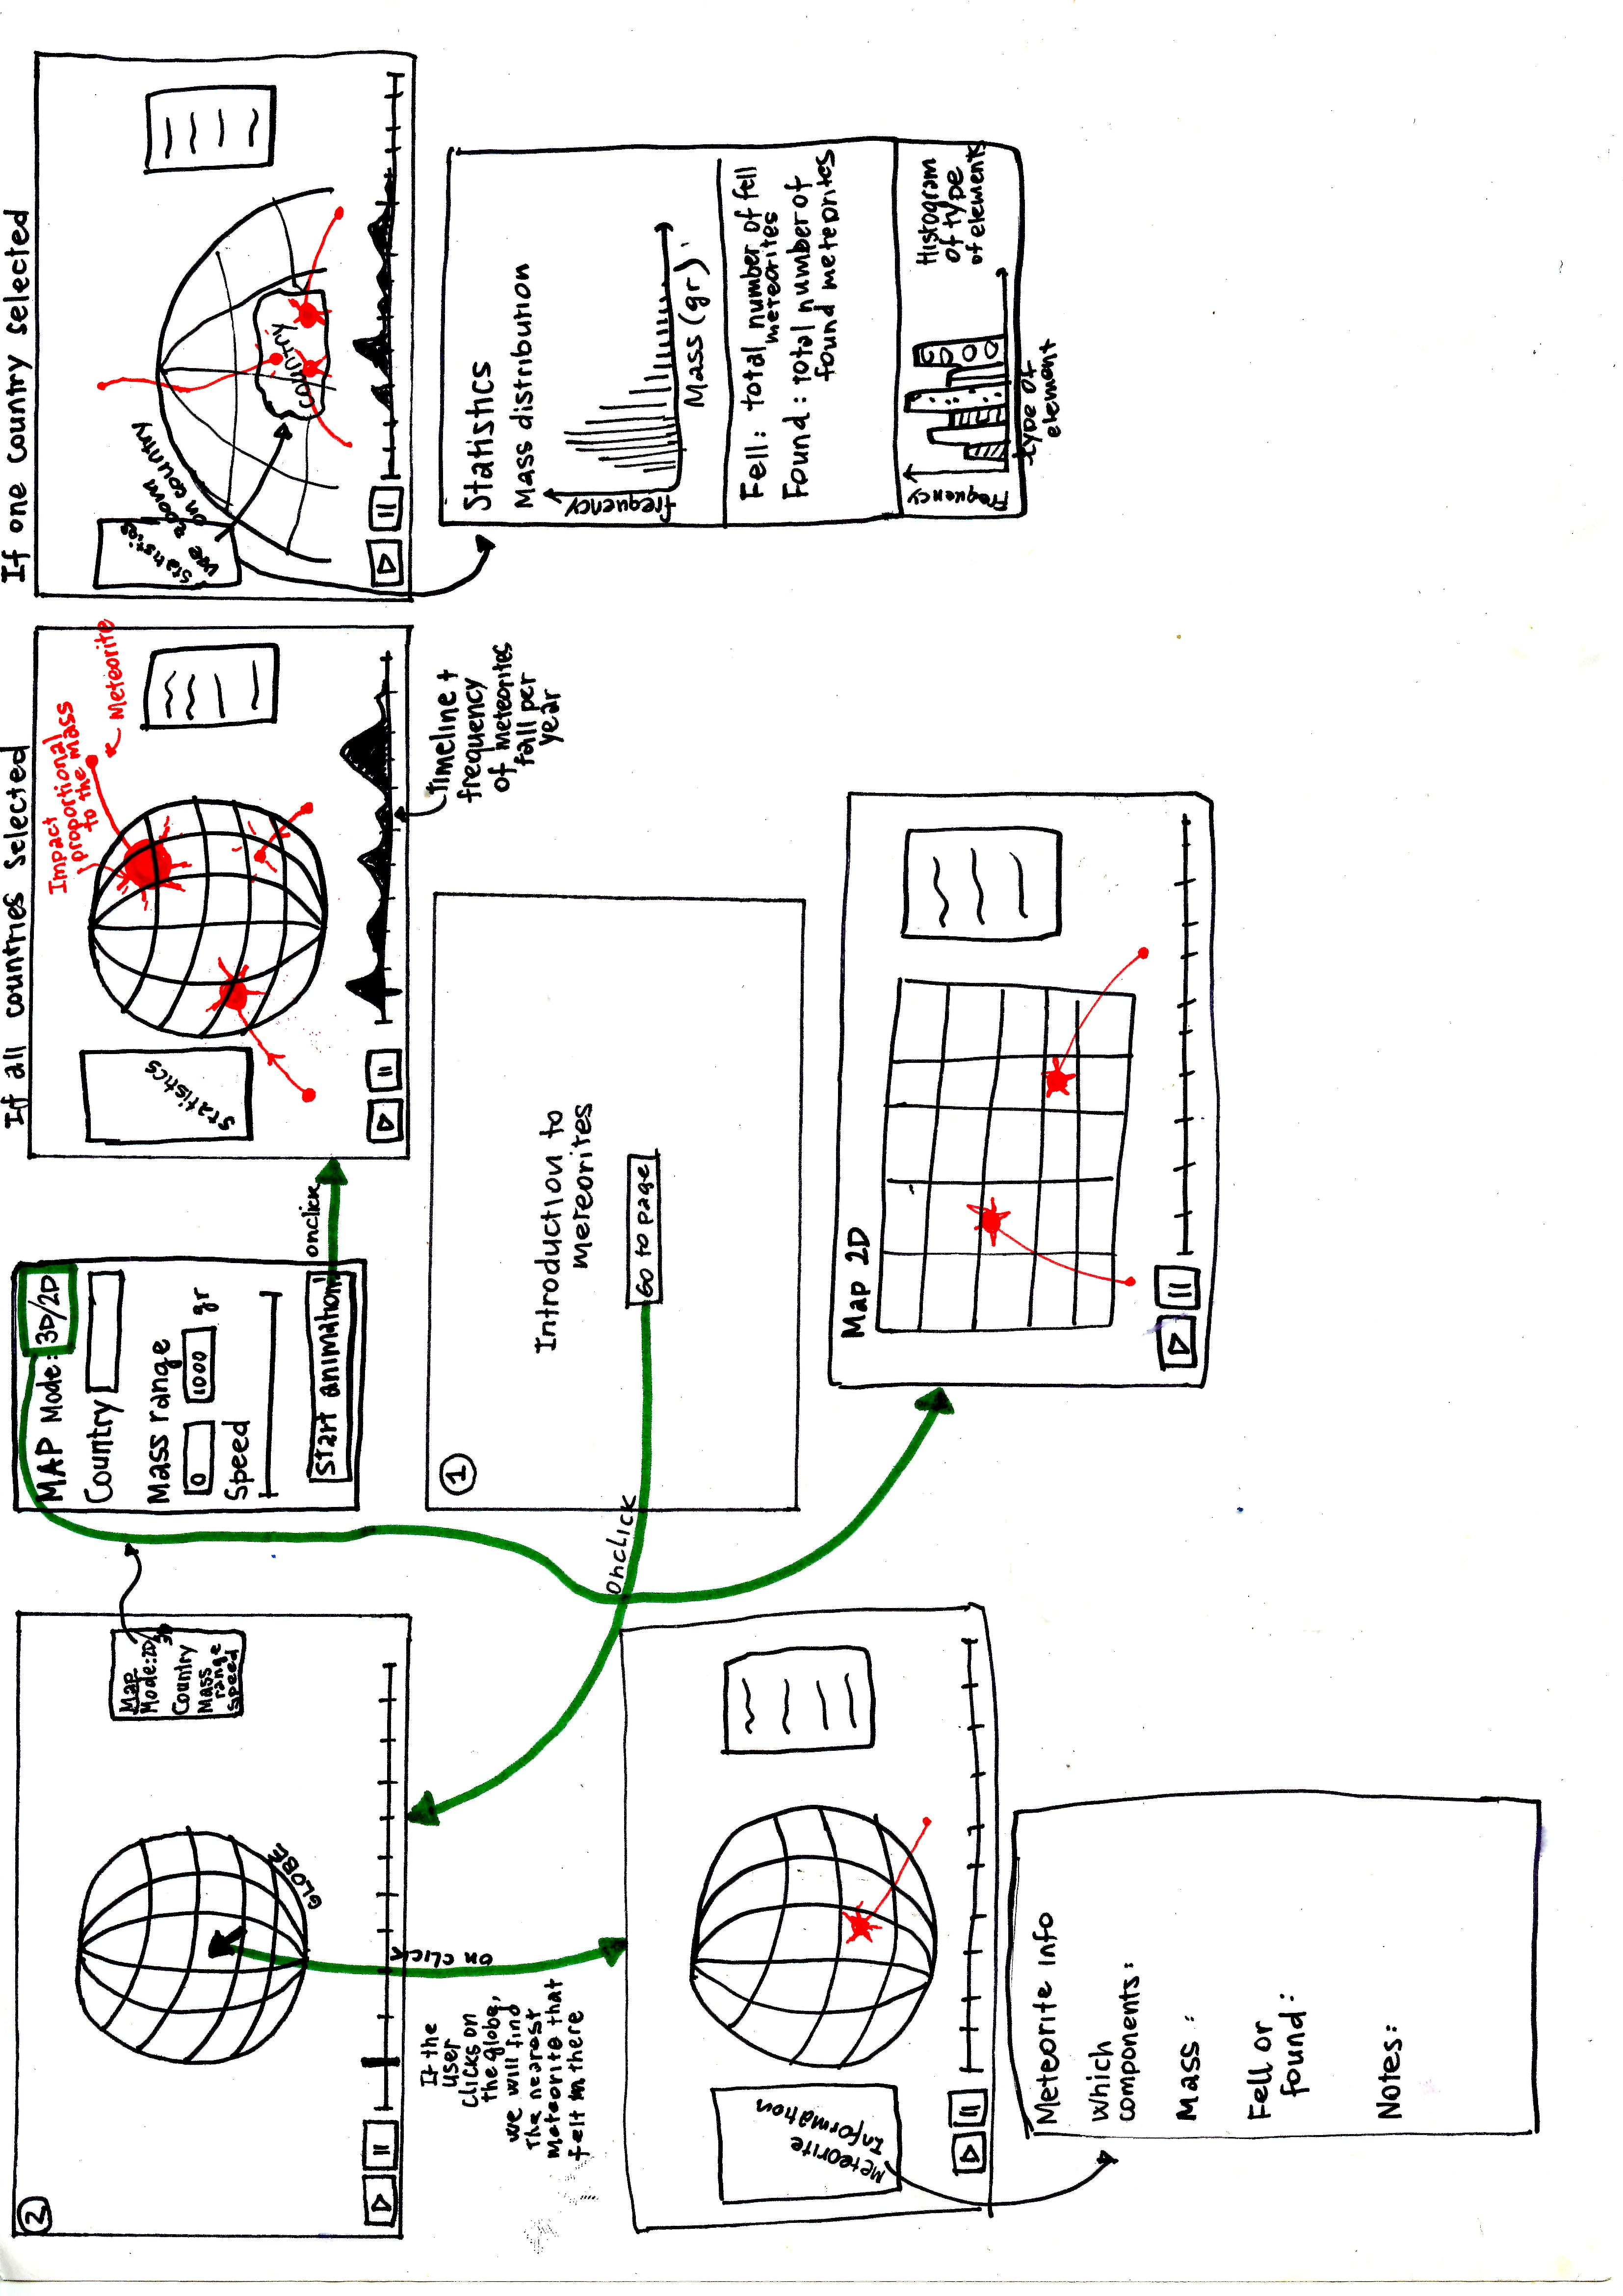
\includegraphics[angle=-90,width=\columnwidth]{images/sketch1.jpg}
  \vspace{-3mm}
  \caption{First sketch of the visualization}
  \label{fig:sketch1}
\end{figure}



\subsection{Globe}
Exploring the Mike Bostock's Blocks \cite{bostock_mike_nodate} we discovered many tutorial allowing the creation of a globe with $d3.js$ \cite{bostock_see-through_nodate,bostock_globe_nodate}.  These works are performed with the \texttt{d3.geo} library that allows an easy way to work with geographic information and different projections.

We then created the globe, but a sticking point came up: how to handle the meteorites' animation with \texttt{d3}?

We then explored other javascript libraries that could handle in a simpler way the animation of 3D objects and we figured out that the \texttt{three.js} library \cite{BibEntry2017Nov} is the most suitable one (explain why).

We inspired our globe from another Mike Bostock example \cite{BibEntry2017Aug} that shows how to import \texttt{geoJSON} files in a \texttt{three.js} scene. The \texttt{three} library doesn't read automatically objects with geometry as \texttt{d3} does. First of all, the \texttt{geoJSON} file containing the countries borders' multilinestring \cite{countryfile} and re-projected the coordinates of the latter into spherical projection. Then, all the starting and ending vertices of the multilinestring have to be pushed in a \texttt{three geometry} and a line has to be drawn between all these couples of vertices.

%Speak about the graticule TODO


A white sphere has been added as well in order to do not see through the globe.
We finally ended up with the following globe:
\begin{figure}[h]
  \centering
  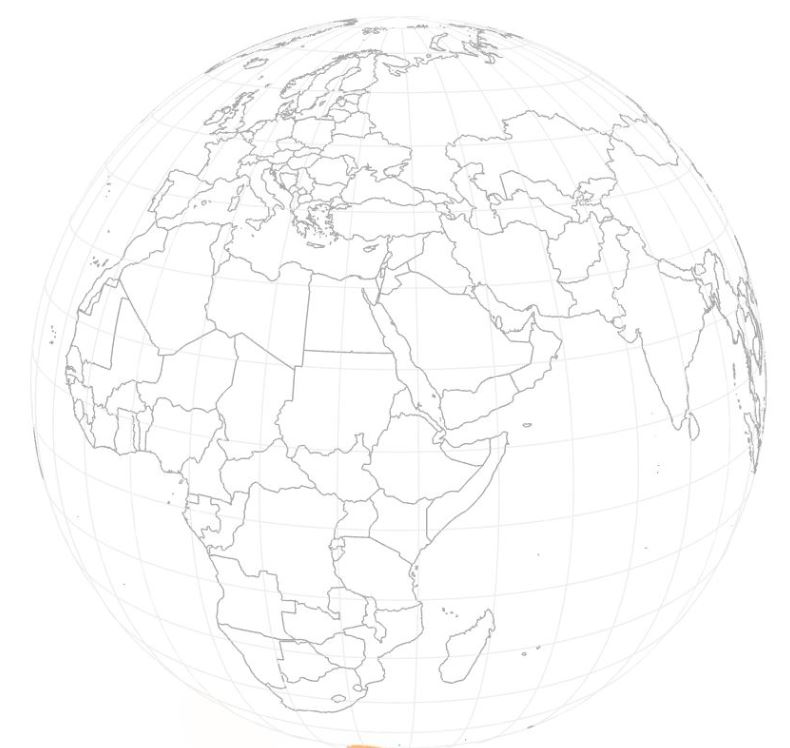
\includegraphics[width=\columnwidth]{images/globe.jpg}
  \vspace{-3mm}
  \caption{Globe with \texttt{three.js}}
  \label{fig:globe}
\end{figure}

In order to add an interaction to the globe, the user can zoom-in, zoom-out, and drag the globe. 
The 2D map has also been taken into account, but being our first aim to make this visualization as realistic as possible, we finally decided to keep only the globe.

\subsection{Meteorites' country}

The original data set provided by Kaggle did not contain any information on countries name. The only way to map a country to a landing was through the geo coordinates. Since the \texttt{csv} file contains many thousands rows, it was impossible to do it manually. This lead us to write a script in python in order to fetch countries based on the tuple (latitude, longitude).

Google Maps, which is likely to be the most famous web app for location, has its services limited to users to avoid DDoS\footnote{Distributed Denial of Service} attack. According to their documentation, the number is limited to a ``a few thousands'' requests by day per person. This could have taken more than one week to get our new data! Clearly, we had to find a solution. That's why we dropped the idea of Google Maps and turned towards Open Street Map, an open source alternative.

Open Street Map also has a system to prevent DDoS attack. But it does not have a limited number of requests per day. Actually their api sends the error $429$ which stands for ``too many requests'', requiring the script to block for several minutes. Eventually the script was run on a server for more than thirty hours.

\subsection{Time-line}

The first idea was to create an animation close to a video. The starting and the ending moments were supposed to be parameters. The inspiration came from \cite{ocks_brush_and_zoom}, parts of the code were taken and adapted to the latest version of ES6\footnote{ECMAScript 6}. There was a plot of the number of meteorites group by year inside the time-line.

\begin{figure}[H]
  \centering
  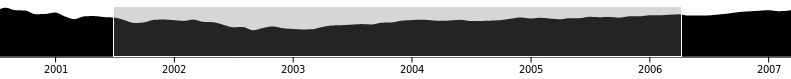
\includegraphics[width=\columnwidth]{images/timeline_brush.png}
  \vspace{-3mm}
  \caption{Time line with a brushing system. Here with fake data.}
  \label{fig:timeline_brush}
\end{figure}

When the application started to work with the globe and the meteorites hitting it. It became obvious selecting the time range was not user friendly. Instead, a flag with the `current' year (of the animation) is moving like a cursor which can be dragged and dropped. This way, only one button to start and stop is needed.

\begin{figure}[H]
  \centering
  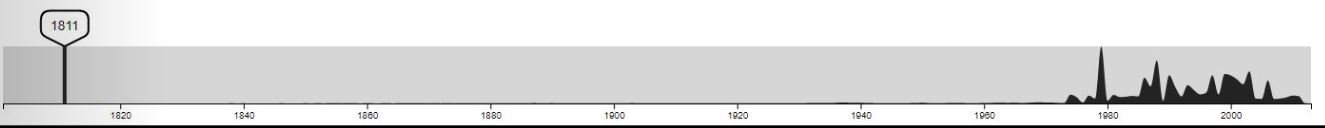
\includegraphics[width=\columnwidth]{images/timeline_original.jpg}
  \vspace{-3mm}
  \caption{Time line with a flag for the year being in the animation.}
  \label{fig:timeline_all_dates}
\end{figure}

The data contains date from $860$ to $2016$. The plot in figure \ref{fig:timeline_all_dates} shows that most meteorites hit the Earth recently. This is unlikely to be the reality. We can interpret it like humans have almost no information on the subject until the 19\textsuperscript{th} century. This information leads us to filter from $1801$ to $2016$.

We had the temporal evolution of the meteorites falls but still did not give any information about the masses of the meteorites. We then decided to add to the initial timeline the average mass per year (Figure \ref{fig:timeline_sketch},\ref{fig:timeline_final_without_label}).

\begin{figure}[H]
  \centering
  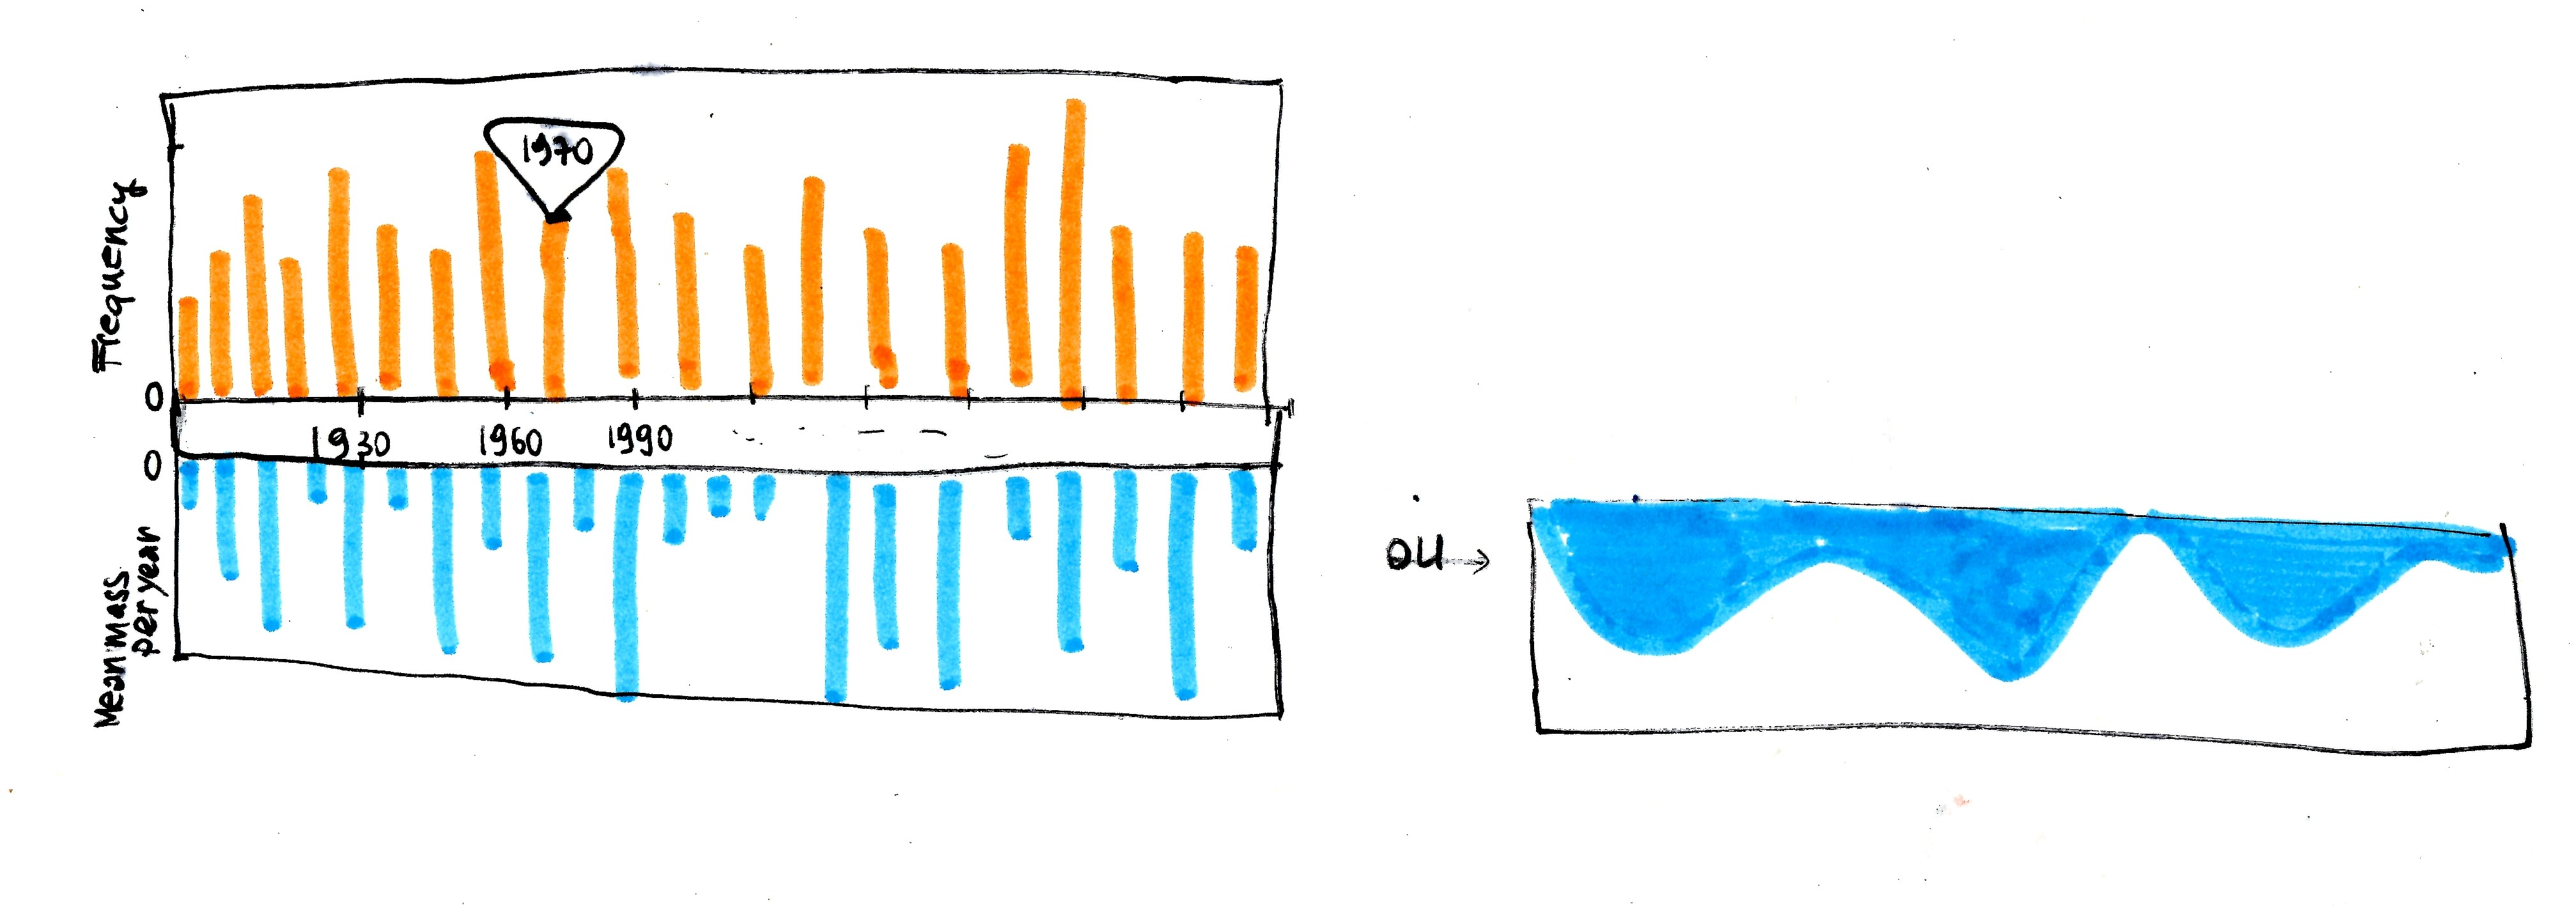
\includegraphics[width=\columnwidth]{images/timeline_sketch}
  \vspace{-3mm}
  \caption{Sketch of time line with the frequency of the meteorite falls per year on the top and average mass per year on the bottom}
  \label{fig:timeline_sketch}
\end{figure}

\begin{figure}[H]
  \centering
  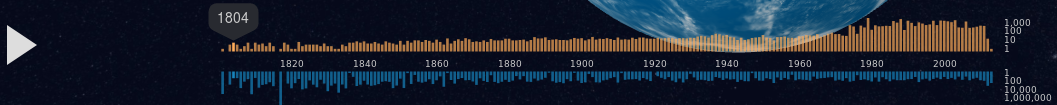
\includegraphics[width=\columnwidth]{images/timeline_final_without_label.png}
  \vspace{-3mm}
  \caption{Time line with plots of frequencies (top top) and average mass (bottom) for each year.}
  \label{fig:timeline_final_without_label}
\end{figure}

The last step was to add labels for vertical axes because the two plots are not intuitive on their own unlike the time axes.

\subsection{Meteorites animation}


\subsection{Search bar}

Users may want to choose and change some parameters like the speed or the dimension of the map (2d vs 3d). The initial version is shown in figure \ref{fig:box_tool}. The opacity was set to $0.5$ in order to let the map (which was not ready at that time) be visible. When the mouse was hover the box, the transparency property was removed as long as the mouse was not outside of it.

\begin{figure}[H]
  \centering
  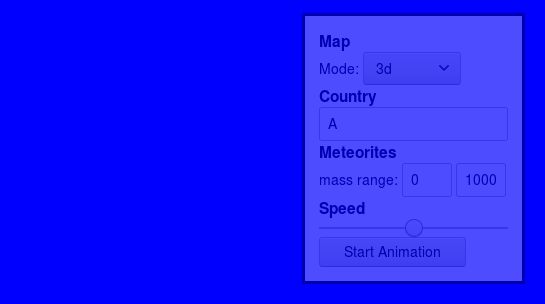
\includegraphics[width=\columnwidth]{images/animation_box_tool.png}
  \vspace{-3mm}
  \caption{The transparent box of parameters of the animation.}
  \label{fig:box_tool}
\end{figure}

The animation of the meteorites falling from the space can be done without much effort in a 3d world. Unfortunately, the 2d version does not allow it. That's why this option was removed.

Since the visualization is intended to a general public, the range of the mass is useless. This option was also removed.

What about the animation speed? Our first feeling was to create something constant over the time. The sparse number of landing per year makes it impossible. Let's assume that we set a constant $\lambda$ for the speed. Since the frequencies of the number of meteorites increases, at some point the number of meteorites in the visualization will reach a threshold which will make the script crashing. If we decrease the value of $\lambda$, then animation would be to slow when the frequency is low. Therefore, the only way to do it is to make $\lambda$ changing depending on the frequency. Thus, the cursor for the \texttt{speed} value was removed too.

Eventually we only kept the country input.

\subsection{Meteorites classification}
At the beginning, the meteorite classification was not taken into account because we did not have any knowledge in the domain, and targeting a general public, it would have been an irrelevant information to present. Going deeper in the domain, we discovered that the type of meteorites depends on the chemical elements of which they are composed by. The attribute \texttt{recclass} presents more than 300 unique classes of meteorites that belong to a defined hierachy well presented in Weisberg et al.  \cite{weisberg_systematics_2006}.
Going up in the nodes of the hierarchy, we ended up with three main classes that describe the material of the meteorites: $stony$, $stony-iron$ and $iron$. 
We firstly checked on the name of the unique classes and classify them by looking at the first letter of \texttt{reclass}. The classification was that easy because the $stony-iron$ meteorites have only two sub-classes ($Pallasite$ and $Mesosiderite$), and the $iron$ meteorites are always classified as $Iron$+$code$. The $stony$ class contains much more sub-classes. Giving that  $iron$ and the $stony-iron$ meteorites contain a limited number of sub-classes, we just checked if the remaining meteorites classes were actually $stony$ (and it was the case!) and assigned to them this class. This simple classification could then draws more attention of the user and make him more familiar with this domain. Indeed, we did not want to go much deeper in the details of the classes because it could have been useless for the public targeted.

Concerning the visualization, the first idea that  came to our mind  was to make a simple bar-chart for every country selected (Figure \ref{fig:sketch1}). 
We soon abandoned this idea because we could have had only a local point of view. In order to do a comparison with the other countries and have a more global point of view, we thought to visualize flows between the type of meteorites and the different countries (Figure \ref{fig:bipartitesketch}). 

\begin{figure}[H]
  \centering
  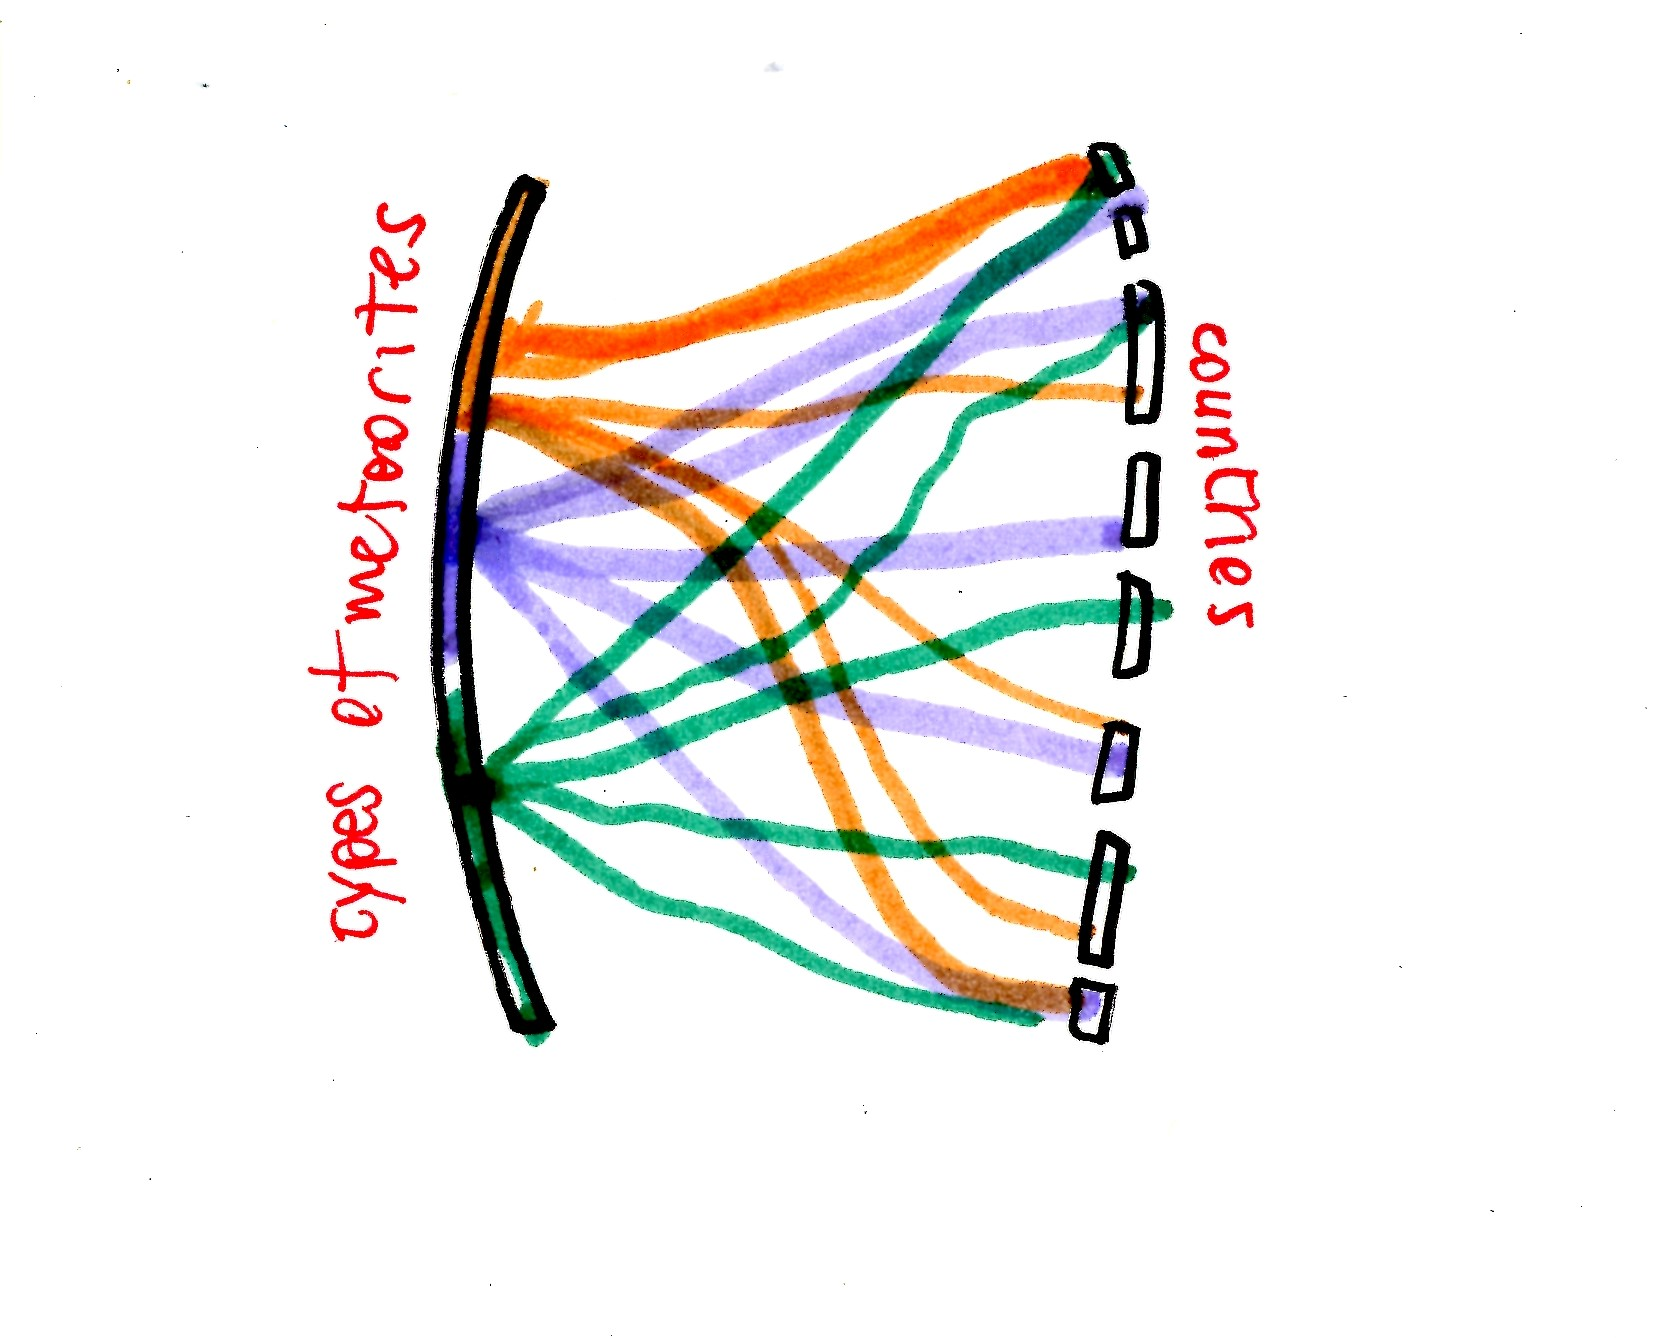
\includegraphics[width=\columnwidth]{images/bipartite}
  \vspace{-3mm}
  \caption{First sketch of the flows between types of meteorites and countries}
  \label{fig:bipartitesketch}
\end{figure}

Firstly we thought to just draw the lines of direct connections between the two different nodes with a constant thickness. We then realised that a thickness depending on the mass would have been more informative. The Sankey diagram came to our mind to vizualize the flows and a nice example proposed by Bremer \cite{BibEntry2017Dec} was our inspiration. Indeed, the latter example propose a bipartite Sankey diagram in the form of a Chord diagram. We discovered a simply way to build a bipartite graph with the \texttt{viz.js} library \cite{bipartite_viz}. This library takes as input parameters the primary key (meteorites' classes), the secondary key (countries) and a value that links the two keys (mass). We first considered all the countries, but we decided to filter out only the countries having a total \texttt{mass} of meteorites bigger than 500 kg and store the other countries as $Others$.


The result of our first bipartite graph was as follow (Figure \ref{fig:bipartite_mass}): 

\begin{figure}[H]
  \centering
  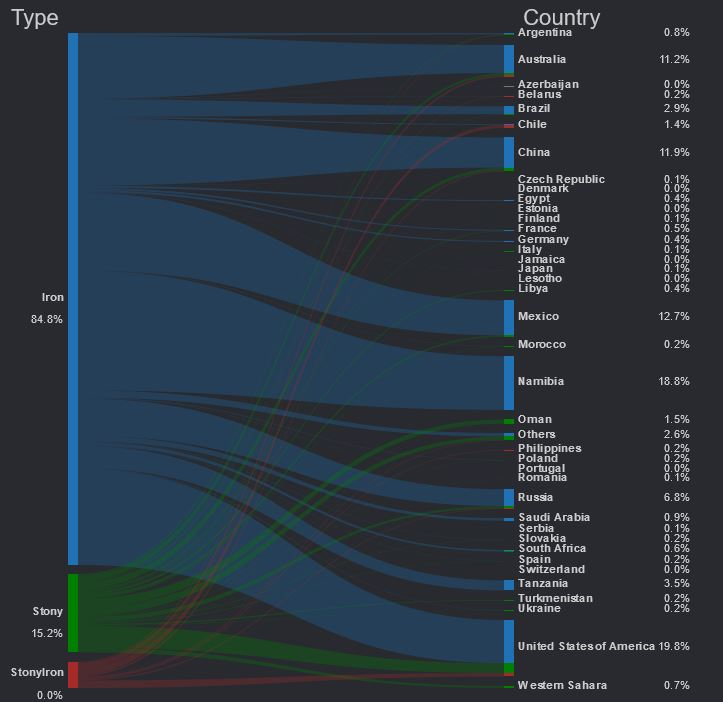
\includegraphics[height=\columnwidth]{images/bipartite_mass}
  \vspace{-3mm}
  \caption{First bipartite graph with thickness of flow depending on the mass}
  \label{fig:bipartite_mass}
\end{figure}

The percentages that you can see on the right of the countries correspond to the sum of all meteorites that fell on that country divided by the mass of all meteorites. If you mouse over a class of meteorite or a country, it will filter out the class selected or the country selected as you can see in figure \ref{fig:bipartite_mouse}. The percentages update dynamically as well.
 
\begin{figure}[H]
  \centering
  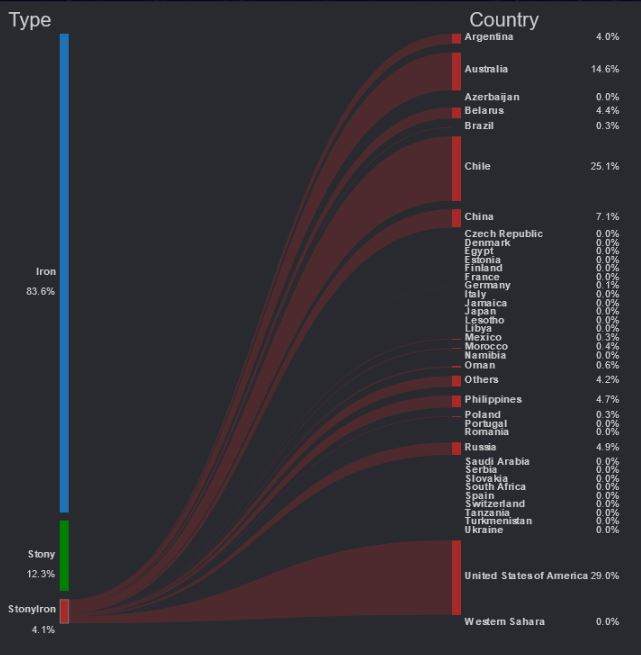
\includegraphics[height=\columnwidth]{images/example_mouse_bipartite}
  \vspace{-3mm}
  \caption{Bipartite graph - on mouse over $stony-iron$ class}
  \label{fig:bipartite_mouse}
\end{figure}

We then noticed that the size of the country biased our first results. In order to do not give a higher weight to the biggest countries, we divided every \texttt{mass} by the area of the country where it fell, obtaining then the \texttt{density} of meteorites by country in $gr/km^{2}$. This time we filtered out the countries having a \texttt{density} bigger than $1$ $gr/km^{2}$ and store the remaining in $Others$.

We ended up with the following graph (Figure \ref{fig:bipartite_density}): 

\begin{figure}[H]
  \centering
  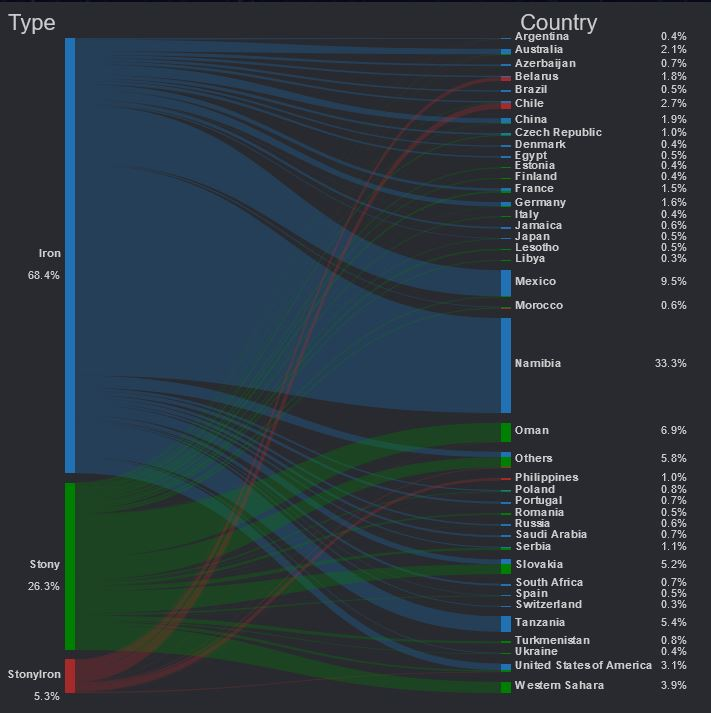
\includegraphics[height=\columnwidth]{images/bipartite_density}
  \vspace{-3mm}
  \caption{Final bipartite graph with thickness of flow depending on the density}
  \label{fig:bipartite_density}
\end{figure}

Countries as Australia, United States and China clearly diminished on importance and Russia was even incorporated to $Others$.

\subsection{Country statistics}
The country statistics panel was from the beginning thought to appear when a country was selected in the search-bar. Hence, we tried to figure out which country's data  could be interesting to visualize. 

Firstly, we decided to visualize the mass distribution of the meteorite falls and finds\footnote{Meteorites are considered falls if they can be
associated with an observed fall event and finds if they
cannot be connected to a recorded fall event \cite{weisberg_systematics_2006}.} and the frequency by meteorite classes (Figure \ref{fig:density_plot}).


\begin{figure}[H]
  \centering
  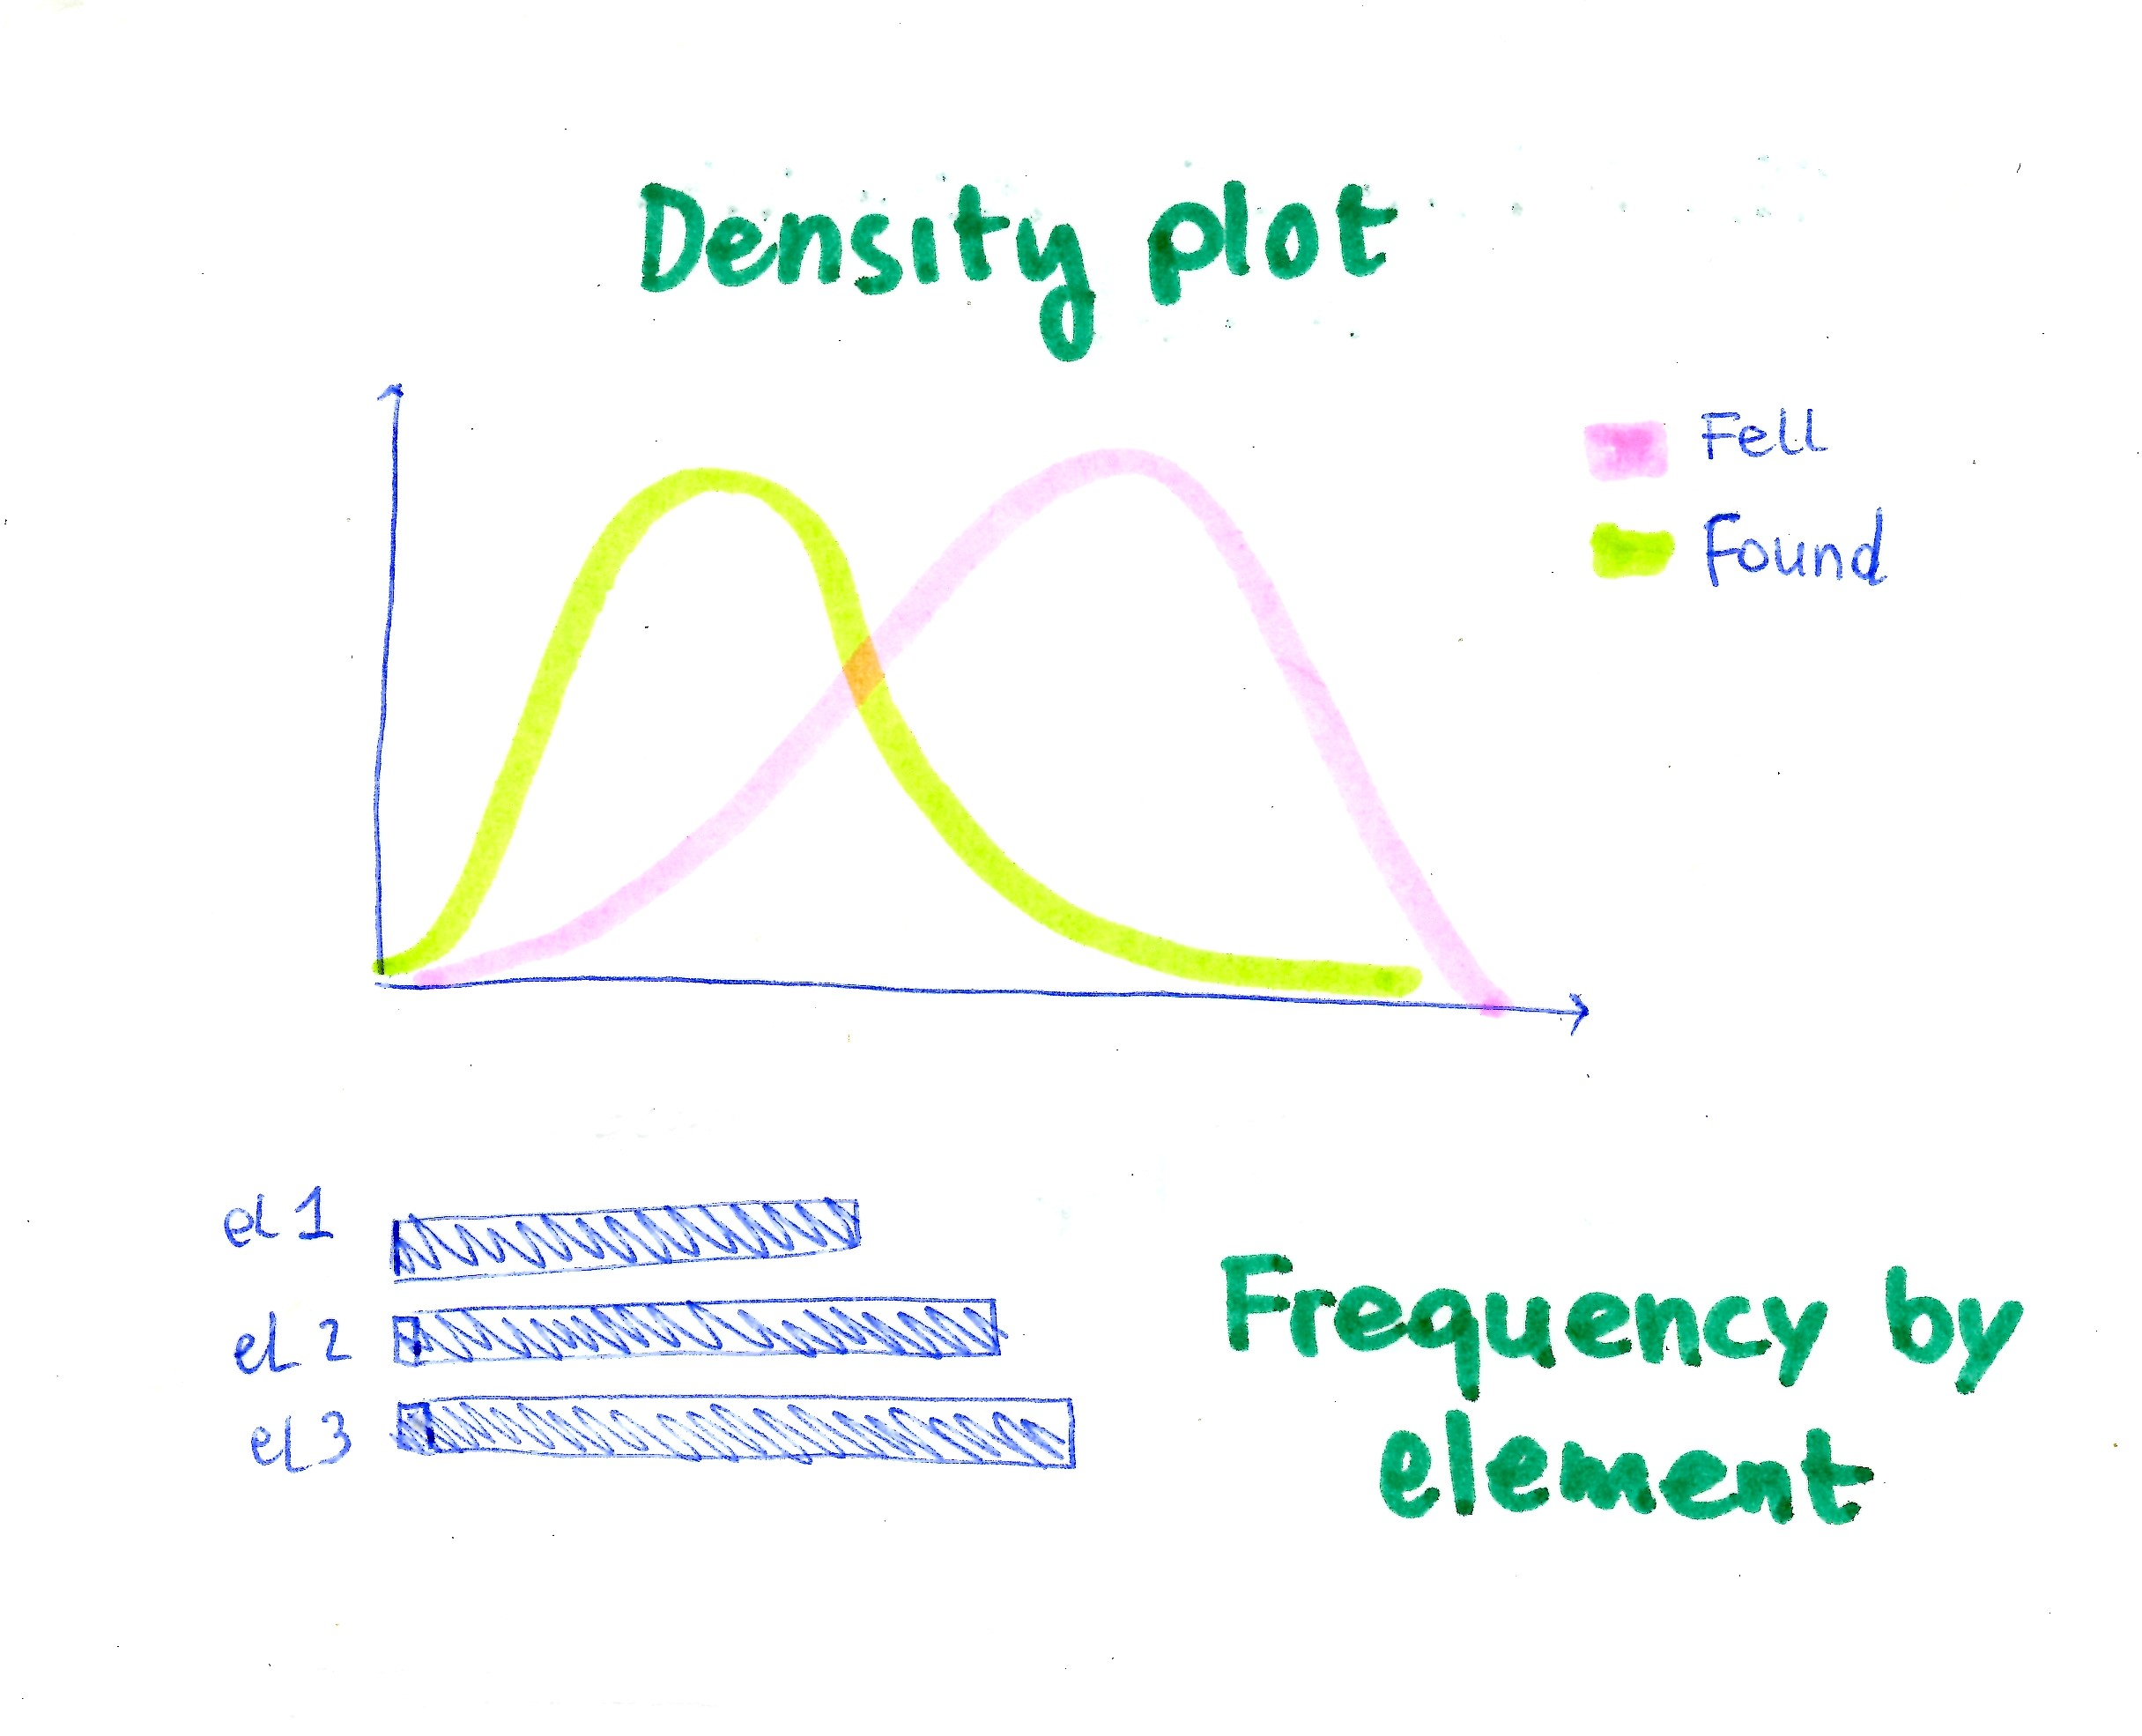
\includegraphics[width=\columnwidth]{images/densityplot}
  \vspace{-3mm}
  \caption{Sketch of density plot and frequency by element}
  \label{fig:density_plot}
\end{figure}


As the information of the meteorite classes was already given with the bipartite graph (Figure \ref{fig:bipartite_density}), the latter option was abandoned. 

Another option that was taken into account was to visualize the three heaviest meteorite recorded that fell in the selected country. A simple text saying the names and the masses of the meteorites was considered a too simple solution; hence, we decided to create a geometry that could remind a meteorite shape as follow:

\begin{figure}[H]
  \centering
  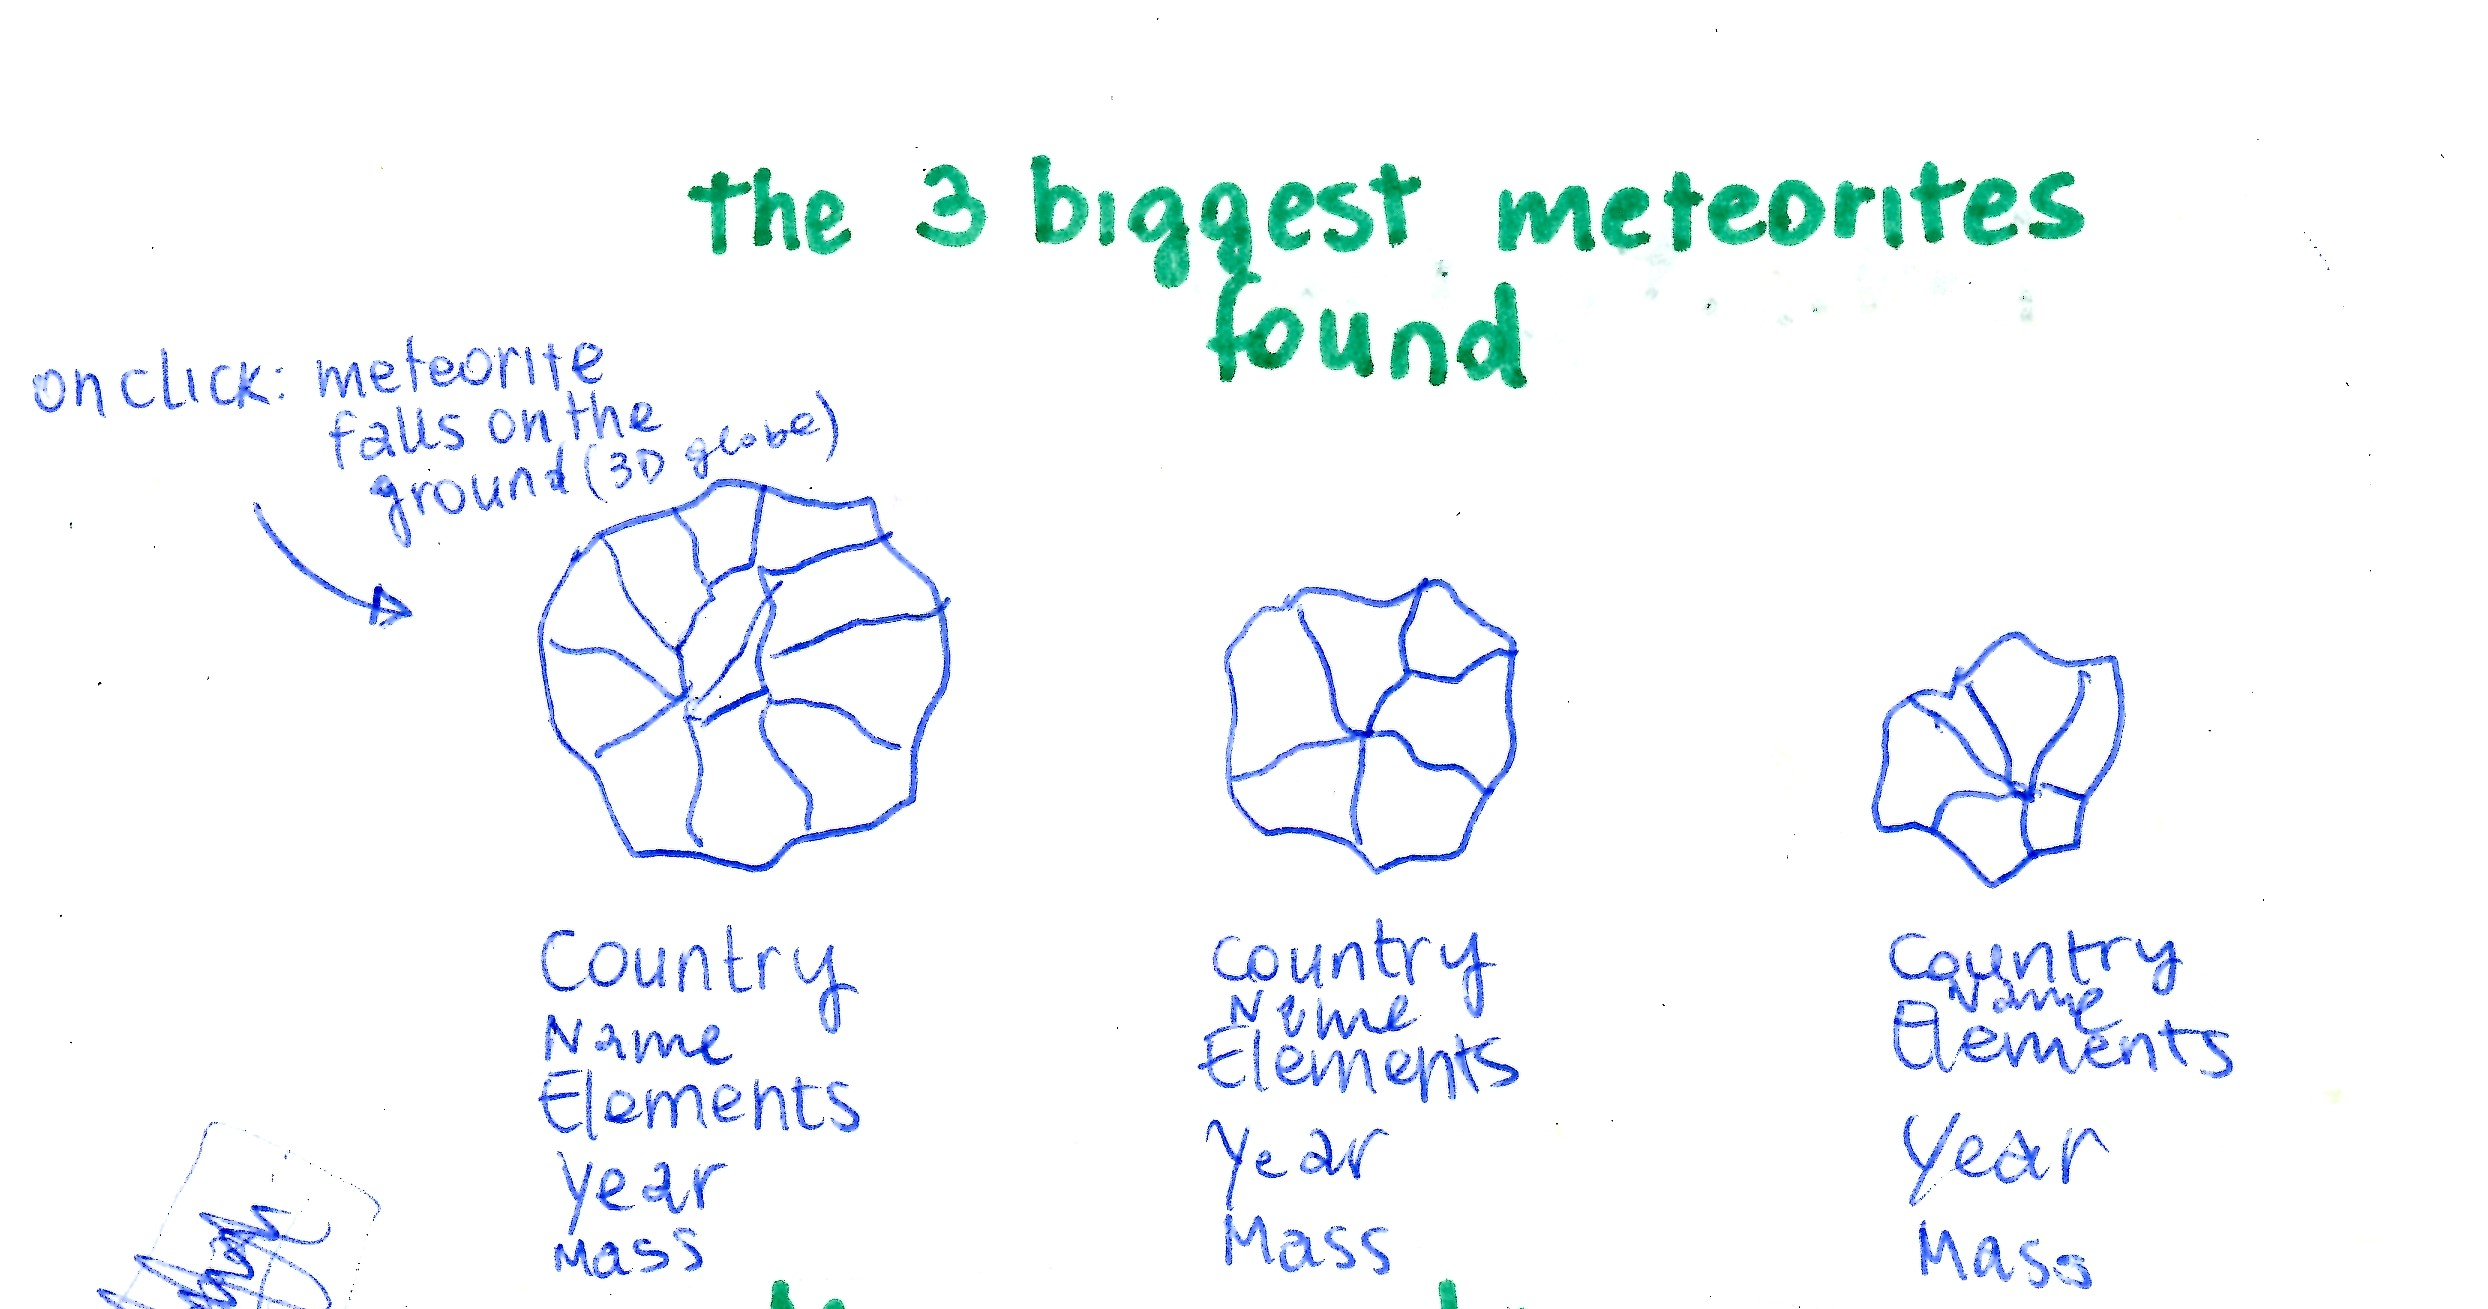
\includegraphics[width=\columnwidth]{images/3biggestmeteorites}
  \vspace{-3mm}
  \caption{Sketch meteorite shape}
  \label{fig:sketch_3_biggest}
\end{figure}

We finally opted to only draw the heaviest meteorite by country giving that most of the countries had only few entries. The library \texttt{three.js} was again the best option to visualize 3D shapes. In order to draw the shape desired, we created a dodecahendrom geometry and pushed random positions to the its vertices. We obtained the following shape: 

\begin{figure}[H]
  \centering
  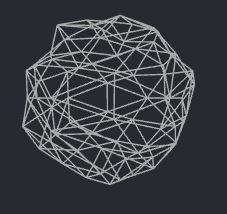
\includegraphics[width=.5\columnwidth]{images/biggestmeteorite}
  \vspace{-3mm}
  \caption{Heaviest meteorite with \texttt{three.js}}
  \label{fig:sketch_biggest}
\end{figure}

Our initial idea was even to click on the meteorite and see the meteorite falling, but this idea was abandoned as well for a lack of time. 


\subsection{Messages}

The International Comet Quarterly publishes a list of all incidents reported related to meteorites \cite{international_comet_quarterly}. We took this data and adapted to make them appear next to the globe. The text does not appear all at once, but word by word. The reason behind is that it is easier to see it when a new message is displayed.

% screen shot here

\subsection{Final touches}
Night-day texture
Layout






\section{Improvements}
\label{sec:improvements}

To do.

\section{Work split}
\label{sec:work_split}

\begin{description}
\item[Rehan Mulakhel] \ \\
  Web page centralizing links to the demo, code and process book. Brushing time line. Dynamic suggestion for the countries. Country to each meteorite based on coordinates. 
\item[Noemi Romano] \ \\
  Data cleaning, globe visualization (partly), country statistics, meteorites classification, ISO codes for countries, getting minimum latitude and longitude for every country to facilitate the zooming on the country selected. 
\item[Raja Soufi] \ \\
  Globe visualization (partly) as well as falling meteorites and world camera animations/movements.
  Improvements to various elements such as timeline and search field, as well as linking the various parts together.
\end{description}




\bibliography{geometeorites}
\bibliographystyle{plain}



\end{document}
